\subsection{CityGen} % (fold)
\label{sec:citygen}
\cite{Kelly2008}

CityGen it's an interactive system that aims  to "rapidly create the urban geometry typical of a modern city". The users can interact and control the generation process. The system, like others, is able to generate road networks that act as foundations to the model. It also can generate buildings but can not achieve the complexity and realism of other systems.


\subsubsection{Road Network} % (fold)
\label{ssub:road_network}


CityGen divided this problem in two steps. First the generation of the "Primary Road Network", and after that, the "Secondary Road Network". This two steps use different methods to generate the roads.
Undirected planar graphs are used to represent all roads. Two graphs for the Primary roads and one for each zone to store the secondary roads.


\emph{Primary Road Generation}

The primary road network uses two graphs, one high level graph that correspond directly to the primary road intersections. It represents the topological structure of the city by it's primary roads, and connections between them. The user is allowed to manipulate this high level graph, to change the high level structure ("topography of the primary road network") of the city .
There is also the low level graph that is generated from the other one, and defines the real path that the roads have in the terrain. It have the same nodes as the first graph and many more, that indicate the points on the terrain which the road passes.
To generate the low level graph it is used "sampling, plotting and interpolation processes".


	

\begin{figure}[htbp]
	\centering
	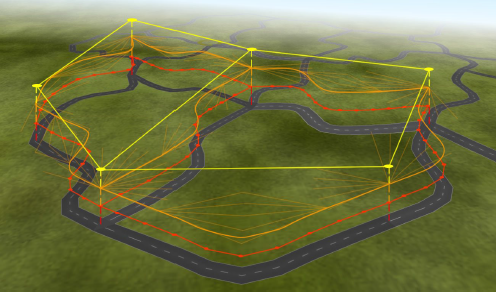
\includegraphics[width=0.95\textwidth]{img/CityGen/RoadGraphs.png}
	\caption{The lighter graph is the High level graph, and the evolution to the darker Low-level graph }
	\label{fig:graphs}
\end{figure}

\emph{Secondary Road Generation}

The author defined city cells as districts, that are the areas of terrain that are enclosed by primary roads. The secondary road network is generated inside this cells using a growth based algorithm similar to the L-Systems technique.

\begin{figure}[htbp]
	\centering
	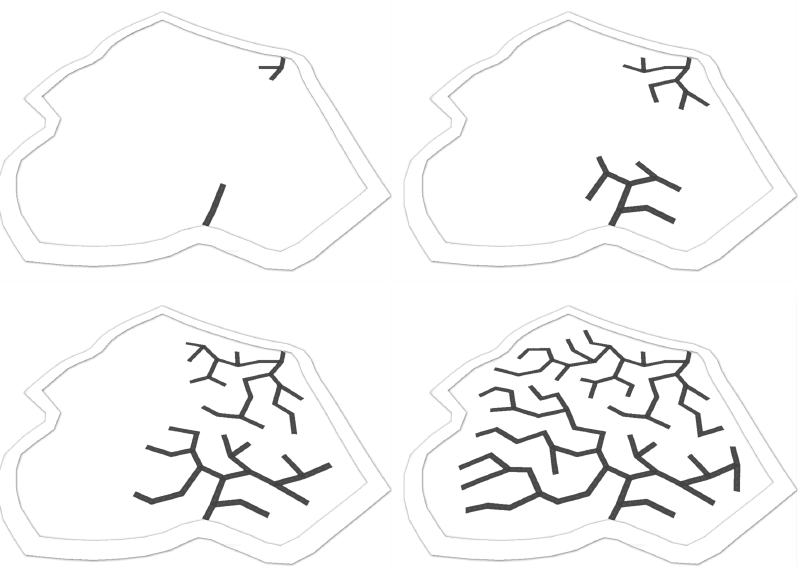
\includegraphics[width=0.95\textwidth]{img/CityGen/SecondaryRoadGrowth.png}
	\caption{}
	\label{fig:graphs}
\end{figure}

% subsubsection road_network (end)


\subsubsection{Buildings} % (fold)
\label{ssub:buildings}



This system generates buildings also. Each building is created in lots that are identified after the extraction of enclosed regions, called blocks, from the secondary graph. Lots that don't have direct access to the roads are excluded. 


Based on the type of block the building footprints are created. After that building geometry is generated by extruding the footprint. The height of each is determined by a height parameter and a noise factor that can be also manipulated. A block is shown in the Figure~\ref{fig:primitiveShapes}, with only primitive shapes.

\begin{figure}[htbp]
	\centering
	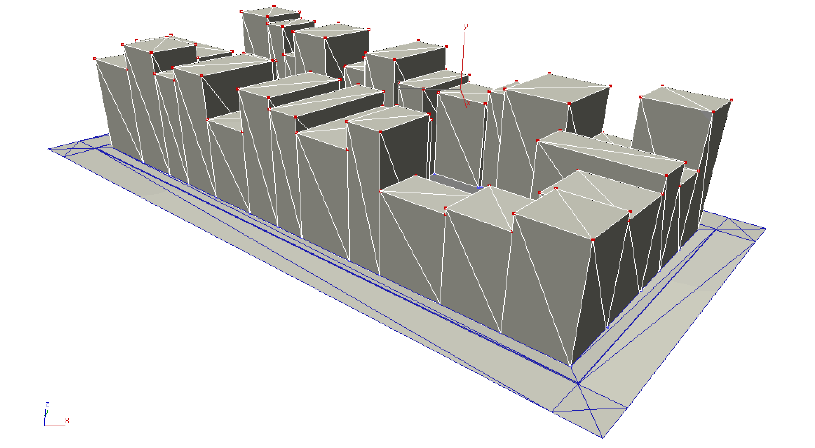
\includegraphics[width=0.95\textwidth]{img/CityGen/BockPrimitiveShapes.png}
	\caption{Primitive Shape Buildings}
	\label{fig:primitiveShapes}
\end{figure}

With this primitive shapes, CityGen uses "advanced materials with shaders to simulate additional geometry".

% subsubsection buildings (end)


% subsection citygen (end)
